\documentclass[11pt]{article}
\usepackage[a4paper,margin=1in]{geometry}
\usepackage{amsmath,amssymb,amsthm,mathtools}
\usepackage{booktabs}
\usepackage{enumitem}
\usepackage{graphicx}
\usepackage{microtype}
\usepackage{hyperref}
\usepackage[nameinlink,capitalise]{cleveref}
\usepackage[numbers,sort&compress]{natbib}

\newtheorem{theorem}{Theorem}[section]
\newtheorem{proposition}[theorem]{Proposition}
\newtheorem{corollary}[theorem]{Corollary}
\newtheorem{lemma}[theorem]{Lemma}
\theoremstyle{definition}
\newtheorem{definition}[theorem]{Definition}
\theoremstyle{remark}
\newtheorem{remark}[theorem]{Remark}
\newcommand{\norm}[1]{\left\lVert#1\right\rVert}
\newcommand{\tr}{\operatorname{tr}}
\newcommand{\Ran}{\operatorname{Ran}}

\title{Reduced Projected-Cross Moment Factorization\\
\large Exact Small-Matrix Closure and a Weak-Mode Conditioning Barrier}
\author{Liang Wang}
\date{July 2026}

\begin{document}
\maketitle

\begin{abstract}
RH-94 carries a source packet through the complete frozen prefix by selecting
four left singular directions of the ambient projected-cross matrix
$K=(I-VV^*)GV$.  This paper asks whether that ambient cross SVD can be
replaced by packet-scale data.

For an orthonormal rank-$r$ packet $V$, put
$A=V^*GV$, $M_j=V^*G^jV$, and $K=(I-VV^*)GV$.  We prove the
projected-cross Gram identity
\[
 K^*K=M_2-A^2
\]
and the cross-cubic identity
\[
 K^*GK=M_3-M_2A-AM_2+A^3.
\]
If $K^*K=R\Sigma^2R^*$ on a positive selected subspace, then
$Q=KR\Sigma^{-1}$ gives the left cross directions,
$V^*GQ=R\Sigma$, and
\[
 Q^*GQ=\Sigma^{-1}R^*(K^*GK)R\Sigma^{-1}.
\]
Hence the complete $(r+k)$-dimensional Ritz matrix is determined by the first
three packet moments, and the ambient cross SVD is algebraically unnecessary.
We also state cutoff reconstruction and separated-projector perturbation
bounds.

The exact reduction exposes a numerical obstruction.  In a 384-bit endpoint
audit of 120 source-seeded updates, the fourth/first cross singular ratio
falls to $2.77\times10^{-11}$; five updates lie below $10^{-8}$.  Normal
equations square this condition number, while the moment identities subtract
nearly equal matrices.  Raw inverse-singular-value reconstruction loses
orthogonality in eight updates, and a binary64 moment-only compression fails a
$10^{-3}$ relative criterion in fifty.  Nevertheless, projecting and
QR-stabilizing the reconstructed directions, followed by direct small Ritz
compression, is tail-stable: all 120 updates agree with the ambient-SVD tail
within a factor $1.000000529$, and all ten RH-94 endpoint gates remain green.

Thus the ambient cross SVD can be removed, but naive moment-only binary64
closure is rejected.  Weak modes must be quotiented or certified by energy,
not inverted blindly.  No all-level conditioning theorem, Hilbert--Polya
operator, zero identification, or Riemann Hypothesis result is claimed.
\end{abstract}

\noindent\textbf{Keywords:} projected-cross Gramian; moment factorization;
normal equations; weak singular mode; Ritz method; validated numerics.

\medskip
\noindent\textbf{MSC 2020:} 47A75; 15A18; 65F15; 65G20; 37C30.

\section{Introduction}

The source-seeded horizon chain of RH-94 replaces late ambient packet resets
by recursive low-dimensional Ritz corrections
\citep{WangSourceSeed2026}.  At each update, however, it computes the leading
left singular directions of
\[
 K=(I-VV^*)GV,
\]
where $G$ is the current positive semidefinite memory Gramian and $V$ is the
incoming rank-$r$ packet.  Although $K$ has only $r$ columns, its left
singular vectors live in the ambient state space.

There are two different reduction questions.
\begin{enumerate}[leftmargin=2em]
\item Can the singular \emph{selection} be performed in $r$ dimensions?
\item Can the entire corrected Ritz matrix be assembled from packet moments,
without an ambient cross SVD?
\end{enumerate}
Both have exact affirmative answers.  The right singular data of $K$ are the
spectral data of $K^*K$, and this matrix is the moment difference
$V^*G^2V-(V^*GV)^2$.  A second identity expresses $K^*GK$ through moments up
to order three.  Together these formulas give the selected complement
directions and every block of the small Ritz compression.

Exact algebra is not the end of the problem.  Forming normal equations squares
the condition number, reconstructing left vectors divides by selected
singular values, and the moment formulas are differences of matrices that can
be individually much larger than the cross terms.  These familiar numerical
hazards \citep{Higham2002,GolubVanLoan2013} become decisive in the archived
chain because the fourth cross mode can be almost null.

The resulting paper has a deliberately mixed conclusion.  The ambient cross
SVD is not structurally necessary: an $r\times r$ factorization plus one
cross-column action suffices, and QR stabilization preserves all tail
certificates.  The stronger claim that binary64 moments alone provide a
stable closure is false on the current data.  This negative branch is useful:
it identifies the precise mode that the next theorem must quotient rather
than recover geometrically.

\section{Exact projected-cross identities}
\label{sec:identities}

Let $G=G^*\ge0$ act on a finite-dimensional Hilbert space $\mathcal K$, and
let $V:\mathbb C^r\to\mathcal K$ be an isometry.  Write
\[
 P=VV^*,\qquad A=V^*GV,\qquad M_j=V^*G^jV,
\]
and define
\begin{equation}
 K=(I-P)GV=GV-VA.
 \label{eq:cross}
\end{equation}

\begin{theorem}[Projected-cross Gram identity]
\label{thm:cross-gram}
The cross normal matrix is
\begin{equation}
 C:=K^*K=M_2-A^2\ge0.
 \label{eq:cross-gram}
\end{equation}
\end{theorem}

\begin{proof}
Since $I-P$ is an orthogonal projector,
\[
 K^*K=V^*G(I-P)GV
 =V^*G^2V-V^*GVV^*GV=M_2-A^2.
\]
Positivity follows from the first expression.
\end{proof}

\begin{theorem}[Cross-cubic identity]
\label{thm:cross-cubic}
The Gramian compressed between cross columns is
\begin{equation}
 N:=K^*GK=M_3-M_2A-AM_2+A^3.
 \label{eq:cross-cubic}
\end{equation}
\end{theorem}

\begin{proof}
Using $K=GV-VA$ and $K^*=V^*G-AV^*$,
\begin{align*}
 K^*GK
 &=(V^*G-AV^*)G(GV-VA)\\
 &=V^*G^3V-V^*G^2VA-AV^*G^2V+AV^*GVA\\
 &=M_3-M_2A-AM_2+A^3.
\end{align*}
\end{proof}

Neither identity asserts that subtractive evaluation is well conditioned.
Indeed, when $K$ is weak, $M_2$ and $A^2$ can be nearly equal even though
each is accurately computed.  The same issue is stronger in
\eqref{eq:cross-cubic}.

\section{Reduced moment factorization theorem}
\label{sec:factorization}

Let the positive selected spectral factor of $C$ be
\begin{equation}
 CR=R\Sigma^2,\qquad R^*R=I_k,\qquad
 \Sigma=\operatorname{diag}(s_1,\ldots,s_k),\qquad s_k>0.
 \label{eq:selected}
\end{equation}
Define
\begin{equation}
 Q=KR\Sigma^{-1}.
 \label{eq:q}
\end{equation}

\begin{theorem}[Reduced moment factorization theorem]
\label{thm:factorization}
The frame $Q$ is an isometry with $Q^*V=0$.  Moreover,
\begin{align}
 V^*GQ&=R\Sigma, \label{eq:bblock}\\
 Q^*GQ&=\Sigma^{-1}R^*NR\Sigma^{-1}. \label{eq:dblock}
\end{align}
Consequently the complete Ritz compression in the orthonormal basis
$Z=[V,Q]$ is
\begin{equation}
 H=Z^*GZ=
 \begin{pmatrix}
 A&R\Sigma\\
 \Sigma R^*&\Sigma^{-1}R^*NR\Sigma^{-1}
 \end{pmatrix},
 \label{eq:h}
\end{equation}
where $C$ and $N$ are determined by $M_1,M_2,M_3$ through
\eqref{eq:cross-gram} and \eqref{eq:cross-cubic}.
\end{theorem}

\begin{proof}
Because $V^*K=0$, one has $V^*Q=0$.  Also
\[
 Q^*Q
 =\Sigma^{-1}R^*K^*KR\Sigma^{-1}
 =I_k.
\]
Next,
\[
 V^*GK=V^*G(GV-VA)=M_2-A^2=C.
\]
Hence
\[
 V^*GQ=CR\Sigma^{-1}=R\Sigma,
\]
which proves \eqref{eq:bblock}.  Equation \eqref{eq:dblock} follows directly
from \eqref{eq:q} and $N=K^*GK$.  Combining the blocks gives
\eqref{eq:h}.
\end{proof}

\begin{corollary}[Ambient cross-SVD removal]
The leading $k$ left singular directions of $K$ and the full
$(r+k)$-dimensional Ritz matrix can be obtained from an $r\times r$ spectral
factorization, packet moments through order three, and the cross-column
reconstruction \eqref{eq:q}.  No singular-value decomposition with an
ambient left factor is algebraically required.
\end{corollary}

\begin{remark}
The ambient action has not disappeared.  Direct formation of $K$ uses $GV$,
and moment formation uses repeated actions of $G$ on $V$.  What disappears is
the ambient \emph{spectral solve}.
\end{remark}

\section{Cutoff stability}
\label{sec:stability}

The inverse $\Sigma^{-1}$ identifies the conditioning immediately.  For a
fixed selected right frame $R$ and fixed positive $\Sigma$, replacing $K$ by
$K+E$ changes the reconstructed frame by
\[
 \widehat Q-Q=ER\Sigma^{-1}.
\]

\begin{proposition}[Reconstruction amplification]
\label{prop:reconstruction}
If $s_k\ge\tau>0$, then
\begin{equation}
 \norm{\widehat Q-Q}_F
 \le \frac{\norm E_F}{\tau}.
 \label{eq:reconstruction-bound}
\end{equation}
\end{proposition}

\begin{proof}
Use $\norm{R\Sigma^{-1}}_2\le\tau^{-1}$ and submultiplicativity.
\end{proof}

The right spectral frame also changes if the cross Gram is perturbed.  Let
$C$ have a squared-singular-value gap
\[
 \gamma=s_k(K)^2-s_{k+1}(K)^2>0.
\]
For a Hermitian perturbation $F$, the Davis--Kahan theorem controls the
selected spectral projectors \citep{DavisKahan1970,StewartSun1990}.

\begin{proposition}[Separated-cutoff projector bound]
\label{prop:projector}
If $2\norm F_2<\gamma$, then, after matching the leading rank-$k$ spectral
clusters,
\begin{equation}
 \norm{\widehat R\widehat R^*-RR^*}_2
 \le \frac{2\norm F_2}{\gamma}.
 \label{eq:projector-bound}
\end{equation}
\end{proposition}

The two estimates expose distinct requirements: the cutoff squared gap
controls the right frame, while the cutoff singular value controls left-frame
reconstruction.  A gap can be adequate even when $s_k$ itself is tiny.

\subsection{Why normal equations are dangerous here}

Suppose $s_1(K)/s_k(K)=\kappa$.  The positive spectrum of $C=K^*K$ has
condition number $\kappa^2$.  At binary64 precision, a ratio
$s_k/s_1\approx10^{-10}$ places the smallest squared mode far below ordinary
relative resolution.  Even if a small-matrix SVD repairs a tiny negative
eigenvalue of a computed $C$, reconstructing $Q$ still amplifies cross-column
error by $10^{10}$.

Moment evaluation adds cancellation indices
\begin{align}
 \chi_2&=\frac{\norm{M_2}_F+\norm{A^2}_F}{\norm C_F},\\
 \chi_3&=\frac{\norm{M_3}_F+\norm{M_2A}_F+\norm{AM_2}_F+\norm{A^3}_F}
 {\norm N_F}.
\end{align}
Large $\chi_j$ do not invalidate the identities; they show why direct
binary64 subtraction may not realize them accurately.

\section{Validated audit}
\label{sec:audit}

\subsection{Protocol}

We replay the 120 width-four source-seeded updates of RH-94
\citep{WangSourceSeed2026}.  At each update we form $K$ but replace its
ambient left SVD by:
\begin{enumerate}[leftmargin=2em]
\item an SVD of the $r\times r$ matrix $K^*K$ as a positive-semidefinite
repair;
\item the reconstruction $Q=KR\Sigma^{-1}$;
\item projection away from $V$ and a thin QR factorization;
\item direct assembly of the stabilized $(r+4)$ Ritz compression.
\end{enumerate}
The direct small compression is used for the primary stabilized chain.  In
parallel, the moment-only matrix \eqref{eq:h} is assembled in binary64 and
compared with its direct counterpart.  The ambient cross-SVD construction is
retained only as a diagnostic comparator.

Tail quadratic forms and endpoint ratios are evaluated with exact binary
inputs in Arb at 384-bit precision \citep{Rump2010}.  The positive route gate
requires every stabilized reduced tail to lie within a factor $1.0001$ of the
ambient-SVD tail and every channel endpoint to remain below the RH-94 ratio
$1.01$.  The negative diagnostics mark
\[
 s_4/s_1<10^{-8},\qquad
 \norm{Q^*Q-I}_2>10^{-6},\qquad
 \frac{\norm{H_{\rm moment}-H_{\rm direct}}_F}
 {\norm{H_{\rm direct}}_F}>10^{-3}.
\]

\subsection{Positive result: tail-stable QR reconstruction}

All 120 stabilized updates are directly Ritz-monotone.  The largest
reduced/ambient-SVD tail ratio is
\[
 1.0000005281,
\]
and all ten endpoints remain green.  The worst endpoint/reference ratio is
$1.001172049$, essentially unchanged from RH-94.  The stabilized packet
orthogonality defect is below $2.77\times10^{-15}$, and the compressed
dimension remains at most $11$.

The selected direction projectors need not be equally close.  Their largest
operator-norm distance is $0.1693$, whereas the largest corrected packet
projector distance is $1.41\times10^{-4}$ and the tail discrepancy is much
smaller still.  Weak directions are therefore geometrically unstable but
energetically almost invisible at these updates.

\subsection{Negative result: moment-only binary64 closure}

Five updates have $s_4(K)/s_1(K)<10^{-8}$, and the minimum ratio is
\[
 2.7686\times10^{-11}.
\]
Raw reconstruction exceeds the orthogonality-failure threshold in eight
updates, reaching a defect $0.9581$.  QR repairs the frame, but it cannot make
the moment subtraction itself accurate.

The binary64 moment compression fails its $10^{-3}$ relative criterion in
fifty of the 120 updates.  The largest compressed-moment relative error is
$6.17\times10^9$, while the cross-cubic relative discrepancy can reach
$1.97\times10^{13}$.  These values reject a naive implementation of
\eqref{eq:h}; they do not contradict the exact identities.

\begin{figure}[t]
\centering
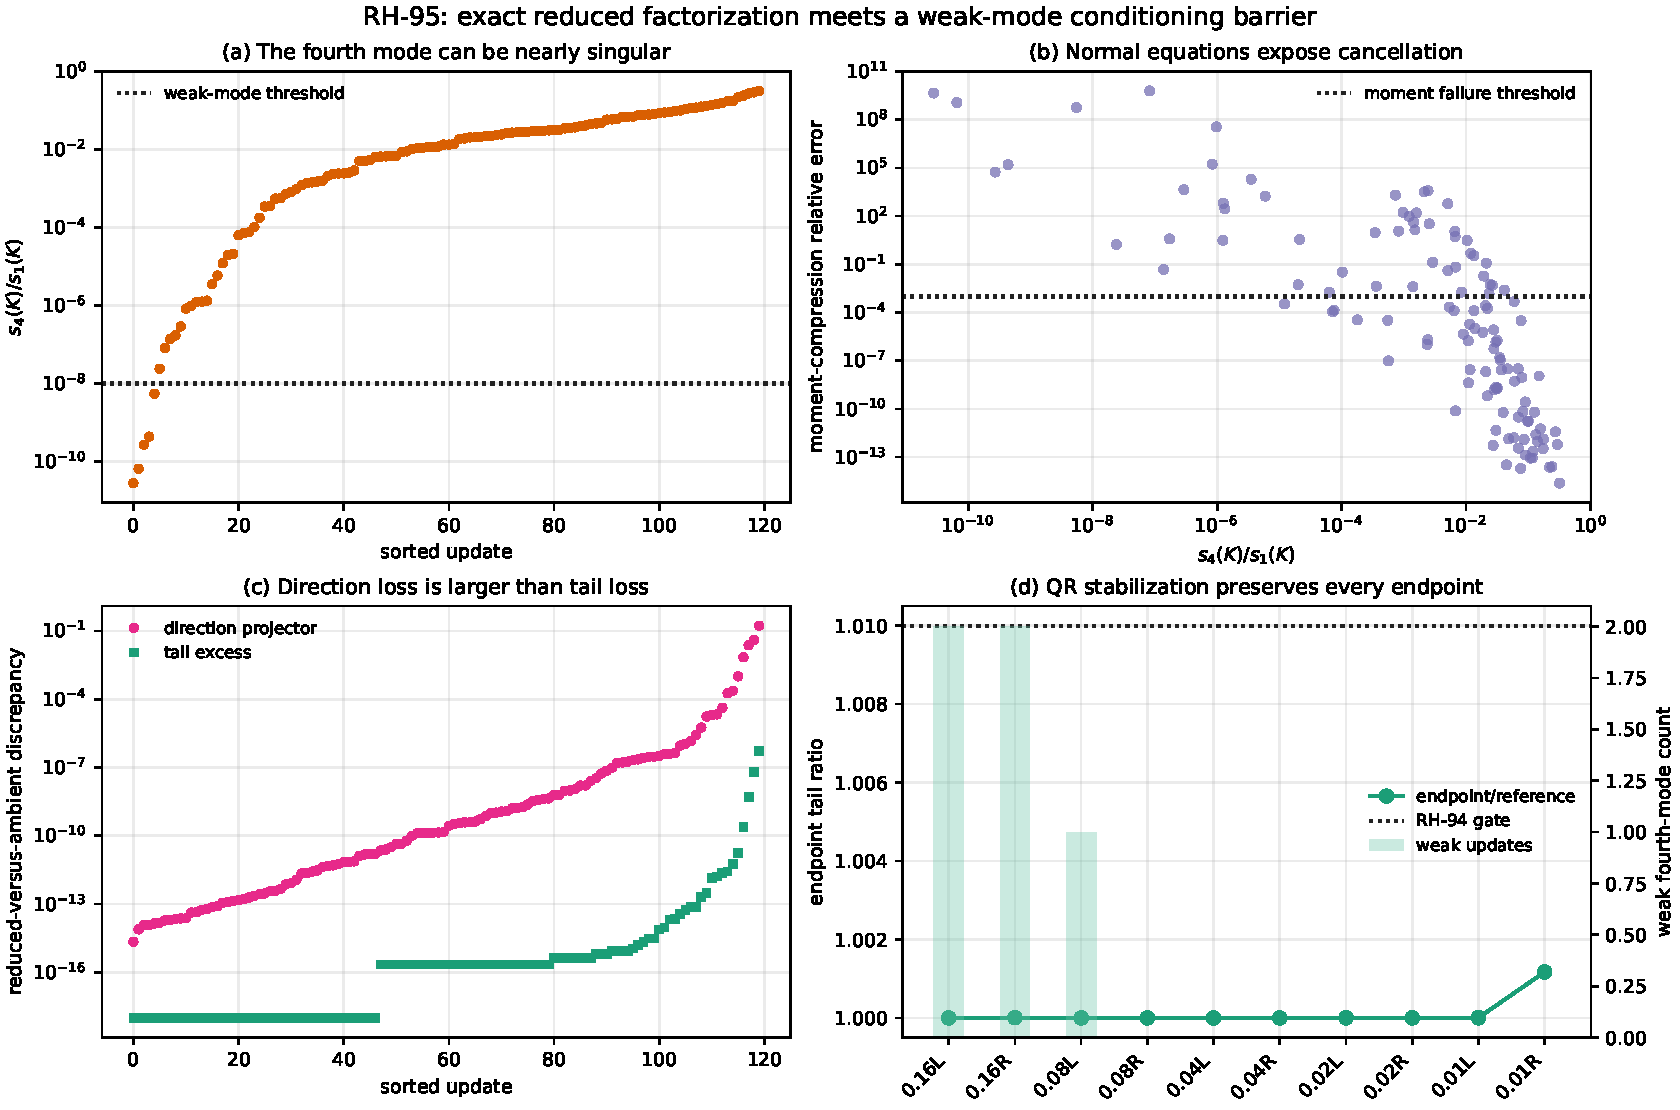
\includegraphics[width=\textwidth]{figures/reduced_cross_moment_factorization.pdf}
\caption{The reduced factorization has two faces.  Weak fourth modes make
normal equations and moment subtraction ill conditioned, yet QR-stabilized
reconstruction preserves all Ritz tail and endpoint gates.}
\label{fig:audit}
\end{figure}

\section{Interpretation: a weak-mode quotient}

The data suggest that demanding a stable geometric fourth direction is the
wrong next goal.  In the weakest updates, many directions can represent the
almost-null cross mode, but the corrected Ritz tail barely changes.  The
relevant equivalence relation should therefore be energetic:
\[
 Q\sim\widetilde Q
 \quad\text{if their corrected rank-$r$ Ritz tails differ by at most a
certified tolerance.}
\]

A future weak-mode quotient theorem should bound the loss caused by
discarding or arbitrarily completing modes below a cutoff.  Such a bound will
need more than discarded cross energy alone.  It should include:
\begin{itemize}[leftmargin=2em]
\item the unselected cross Frobenius energy;
\item a gap or residual for the leading rank-$r$ compressed Ritz cluster;
\item the complement diagonal energy available in omitted directions;
\item the current tail scale, so the statement is relative to the target.
\end{itemize}
If this bound is small, the chain may use adaptive width and avoid inversion
of numerically meaningless singular modes.

\section{Claim boundary}

The exact projected-cross Gram identity and reduced moment factorization
theorem are finite-dimensional algebraic results.  The audit additionally
supports QR-stabilized tail equivalence on ten frozen channels.  It does not
establish:
\begin{enumerate}[leftmargin=2em]
\item stable binary64 moment-only closure---the archived experiment rejects
that claim;
\item a uniform positive lower bound for the fourth cross singular value or
its squared gap;
\item an analytic weak-mode quotient or adaptive-width theorem;
\item removal of the ambient actions needed to form $GV$, $G^2V$, or $G^3V$;
\item repeated all-level block contraction, the normalization/observability
bridge, a Hilbert--Polya operator, zeta-zero identification, or the Riemann
Hypothesis.
\end{enumerate}

\section{Conclusion}

The projected-cross step has an exact small-matrix closure.  Its right
singular data are carried by $M_2-A^2$, its complement Gram block is carried
by moments through order three, and the ambient cross SVD can be replaced by
an $r\times r$ factorization plus reconstruction.  With projection and QR
stabilization, this replacement preserves every audited tail and endpoint
certificate.

The same calculation reveals why a stronger moment-only claim would be
premature.  The fourth cross mode can be ten orders of magnitude below the
first, so normal equations, inverse-singular reconstruction, and subtractive
moment formulas encounter severe conditioning.  The next layer should not
try to identify this weak direction more accurately.  It should prove that
weak cross modes can be quotiented by a certified tail-loss bound.

\bibliographystyle{plainnat}
\bibliography{references}

\end{document}
